\section{The regionally proximal relation}

\begin{frame}
  \begin{definition}[regionally proximal relation]
    \label{def:rpr}
    Let $(X, T)$ be a TDS.
    Two points $x,y \in X$ are called \emph{regionally proximal}
    if for each $\varepsilon > 0$ there exist $x' \in B_\varepsilon(x), y' \in B_\varepsilon(y)$
    and $t \in T$ such that $d(tx', ty') < \varepsilon$.
    We denote the set of regionally proximal pairs by $Q_2(X) \subseteq X \times X$.
  \end{definition}

  \begin{center}
    \begin{tikzpicture}[scale = 1.4]
  % Coordinates of the main points
  \coordinate (A) at (2,3);
  \coordinate (B) at (4,1.5);

  % Off-center lighter points initial positions
  \coordinate (Alight) at ($(A) + (5pt,2pt)$);
  \coordinate (Blight) at ($(B) + (-5pt,-2pt)$);

  % Midpoint of lighter points
  \coordinate (Mid) at ($0.5*(Alight) + 0.5*(Blight)$);

  % Meeting point shifted 2 cm to the right of Mid
  \coordinate (M) at ($(Mid) + (2cm,0)$);

  % Draw dotted circles around main points
  \draw[dotted, thick] (A) circle (10pt);
  \draw[dotted, thick] (B) circle (10pt);

  \node[red, above left] at (A) {$x$};
  \node[blue, below right] at (B) {$y$};

  % Draw main points (smaller)
  \fill[red] (A) circle (2pt);
  \fill[blue] (B) circle (2pt);

  % Draw lighter points at initial positions
  \fill[red!50] (Alight) circle (1.5pt);
  \fill[blue!50] (Blight) circle (1.5pt);

  \node[red!50, above right] at (Alight) {$x'$};
  \node[blue!50, below left] at (Blight) {$y'$};

  % Draw trajectories of lighter points toward the meeting point
  \draw[red!50, thick, ->] (Alight) to[out=0,in=145] ($(M) + (0, 0.2)$);
  \draw[blue!50, thick, ->] (Blight) to[out=0,in=-145] (M);

  % Draw meeting point
  \draw[dotted, thick] (M) circle (10pt);

\end{tikzpicture}
  \end{center}
    
\end{frame}

\begin{frame}

  \begin{definition}[regionally proximal relation]
    \label{def:rpr}
    Let $(X, T)$ be a TDS.
    Two points $x,y \in X$ are called \emph{regionally proximal}
    if for each $\varepsilon > 0$ there exist $x' \in B_\varepsilon(x), y' \in B_\varepsilon(y)$
    and $t \in T$ such that $d(tx', ty') < \varepsilon$.
    We denote the set of regionally proximal pairs by $Q_2(X) \subseteq X \times X$.
  \end{definition}
  Equivalently: There is $(x_n)$, $(y_n)$ in $X$ and $(t_n)$ in $T$, s.t.
  \begin{equation*}
      \label{eq:rprchar}
      x_n \to x, \ y_n \to y \ \text{and} \ d(t_n x_n, t_n y_n) \to 0.
  \end{equation*} 
  and
  \begin{equation*}
    Q_2(X) = \bigcap_{U \in \mathcal{U}(\Delta(X))} \overline{TU} 
  \end{equation*}
  with $\Delta(X) = \{(x, x) \ | \ x \in X\}$ the diagonal in $X \times X$.
\end{frame}

\begin{frame}
\begin{theorem}
  The regionally proximal relation is closed, invariant, symmetric and reflexive.
\end{theorem}

\begin{enumerate}
  \item symmetric and reflexive by definition
  \item closed, since intersection of closed sets
  \item invariant: $(x, y) \in Q_2(X)$, i.e. $d(t_n x_n, t_n y_n) \to 0$ then $d(t_n t_0^{-1} t_0 x_n, t_n t_0^{-1} t_0 y_n) \to 0$.
\end{enumerate}

Not transitive in general! See Example.
\end{frame}

\begin{frame}
  \begin{columns}
  \column{0.5\textwidth}
  \only<1>{%
  Let $X = [0, 2]$ and $T = \mathbb{R}$.
  Then the following map is an $\mathbb{R}$-action on $[0, 2]$
  and defines a TDS.

  \begin{align*}
    &\mathbb{R} \times [0, 2] \to [0, 2] \\
    &(t, x) \mapsto
    tx := \begin{cases}
      0 & x = 0 \\
      \frac{1}{1 + (\frac{1}{x} - 1)e^{-t}} & x \in (0, 1] \\
      \frac{1}{1 + (\frac{1}{x - 1} - 1)e^{-t}} + 1 & x \in (1, 2]
    \end{cases}
  \end{align*}
  }%
  \only<2->{%
  Every point greater $0$ and smaller $1$ tends to $1$ 
  and every point greater $1$ tends to $2$ with $t \to \infty$.
  }

  \only<3->{%
  We also observe that $\{0\}$, $\{1\}$ and $\{2\}$ are closed invariant.
  }
  \column{0.5\textwidth}
  
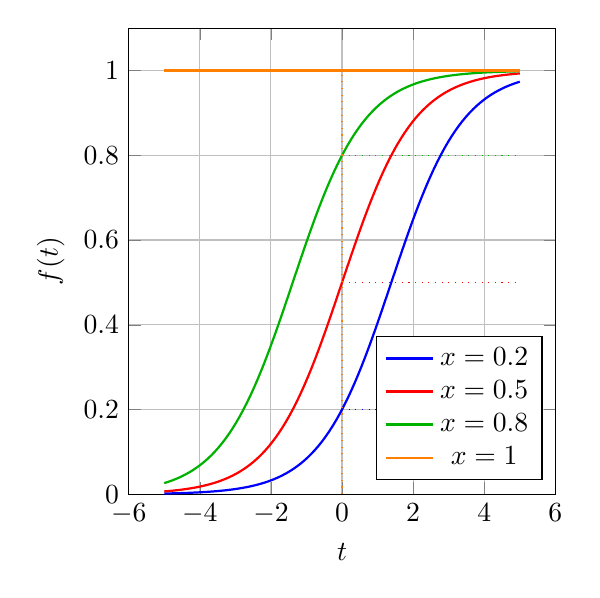
\begin{tikzpicture}[scale=1]
  \begin{axis}[
      domain==3:3,
      samples=100,
      xlabel={$t$},
      ylabel={$f(t)$},
      grid=major,
      ymin=0, ymax=1.1,
      legend pos=south east,
      width=7cm, height=7.5cm,
    ]

    % Values of x
    \def\xA{0.2}
    \def\xB{0.5}
    \def\xC{0.8}
    \def\xD{1}

    % Plot for x=0.2
    \addplot[blue, thick] {1/(1 + ((1/\xA)-1)*exp(-x))};
    \addlegendentry{$x=0.2$}
    % Dotted vertical line at t=0 from 0 to f(0)=x
    \draw[blue, dotted] (axis cs:0,0) -- (axis cs:0,\xA);
    % Dotted horizontal line at y=f(0)=x from t=0 to t=5
    \draw[blue, dotted] (axis cs:0,\xA) -- (axis cs:5,\xA);

    % Plot for x=0.5
    \addplot[red, thick] {1/(1 + ((1/\xB)-1)*exp(-x))};
    \addlegendentry{$x=0.5$}
    \draw[red, dotted] (axis cs:0,0) -- (axis cs:0,\xB);
    \draw[red, dotted] (axis cs:0,\xB) -- (axis cs:5,\xB);

    % Plot for x=0.8
    \addplot[green!70!black, thick] {1/(1 + ((1/\xC)-1)*exp(-x))};
    \addlegendentry{$x=0.8$}
    \draw[green!70!black, dotted] (axis cs:0,0) -- (axis cs:0,\xC);
    \draw[green!70!black, dotted] (axis cs:0,\xC) -- (axis cs:5,\xC);

    % Plot for x=1
    \addplot[orange, thick] {1/(1 + ((1/\xD)-1)*exp(-x))};
    \addlegendentry{$x=1$}
    \draw[orange, dotted] (axis cs:0,0) -- (axis cs:0,\xD);
    \draw[orange, dotted] (axis cs:0,\xD) -- (axis cs:5,\xD);

  \end{axis}
\end{tikzpicture}

  \end{columns} 
\end{frame}

\begin{frame}
  \begin{columns}
    \column{0.5\textwidth}
    Consider the system from the previous slide.

    The pairs $(0, 1)$ and $(1, 2)$ are regionally proximal.

    But $(0, 2)$ is not a regionally proximal pair.

    \column{0.5\textwidth}
    For $0$ and $1$ we have:
    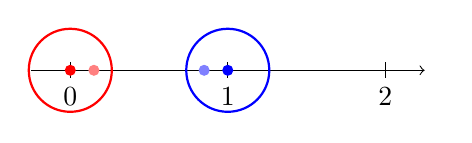
\begin{tikzpicture}
  \draw[->] (-0.5,0) -- (4.5,0) node[right] {};
  % Draw ticks and labels
  \foreach \x in {0,1,2} {
    \draw (2*\x,0.1) -- (2*\x,-0.1) node[below] {\x};
  }

  \draw[thick, red] (0,0) circle (15pt);
  \fill[red] (0,0) circle (2pt);
  \fill[red!50] (0.3,0) circle (2pt);

  \draw[thick, blue] (2,0) circle (15pt);
  \fill[blue] (2,0) circle (2pt);
  \fill[blue!50] (1.7,0) circle (2pt);
\end{tikzpicture}
    With $t$ large enough:
    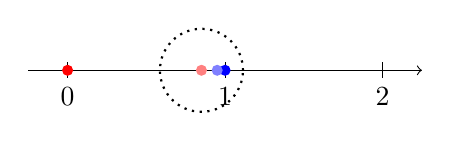
\begin{tikzpicture}
  \draw[->] (-0.5,0) -- (4.5,0) node[right] {};
  
  % Draw ticks and labels
  \foreach \x in {0,1,2} {
    \draw (2*\x,0.1) -- (2*\x,-0.1) node[below] {\x};
  }

  \fill[red] (0,0) circle (2pt);
  \fill[red!50] (1.7,0) circle (2pt);

  \fill[blue] (2,0) circle (2pt);
  \fill[blue!50] (1.9,0) circle (2pt);

  \draw[thick, dotted] (1.7,0) circle (15pt);
\end{tikzpicture}

  \end{columns}
\end{frame}

\begin{frame}
\begin{proposition}
  \label{prop:phiSqQ2XcQ2Y}
  Let $\varphi : (X,T) \to (Y,T)$ a factor. Then $(\varphi \times \varphi) (Q_2 (X)) \subseteq Q_2(Y)$.
\end{proposition}
\pause
\begin{theorem}
  Let $(X,T)$ a TDS and $\varphi : (X,T) \to (Y,T)$ an equicontinuous factor.
  Let $R_\varphi$ the ICER generated by $\varphi$. Then $Q_2(X) \subseteq R_\varphi$.
\end{theorem}
Proof by contradiction using the invariant metric.
\pause
\begin{corollary}
 Let $(X, T)$ be an equicontinuous TDS.
  Then $Q_2(X) = \Delta(X)$.
\end{corollary}
The identity map with $\Delta(X)$ as ICER is an equicontinuous factor.
\end{frame}

\begin{frame}
  Since the MEF is an equicontinuous factor, we have
  \begin{corollary}
    Let $(X, T)$ be a TDS and $R_\text{MEF}$ the ICER generated by the MEF.
    Then $Q_2(X) \subseteq R_\text{MEF}$.
  \end{corollary}
  Do we also have $R \subseteq Q_2(X)$?
\end{frame}

\begin{frame}
  But first:
  \begin{definition}[topologically weakly mixing]
    Let $(X,T)$ be a TDS. Then $(X,T)$ is called \emph{weakly mixing} if every non-empty, $T$-invariant and open $U\subseteq X \times X$ is dense in $X \times X$.
  \end{definition}
  \pause
  \begin{proposition}[weakly mixing systems have trivial $Q_2$]
    Let $(X,T)$ be a weakly mixing TDS. Then $Q_2(X) = X \times X$.
  \end{proposition}
  Using the theorem of Baire and the characterization of the
  regionally proximal equation using intersections.
  \pause
  \begin{corollary}[MEF of weakly mixing system]
    The MEF of a weakly mixing system is trivial.
  \end{corollary}
  Since $Q_2(X) = X \times X \subseteq R_\text{MEF}$.
\end{frame}

\begin{frame}
  \begin{minipage}{0.45\textwidth}
    \begin{center}
      $(X, T)$ equicontinuous
      \vspace{2em}
      \begin{enumerate}
        \item MEF is the identity map, biggest possible factor
        \only<2->{\item $Q_2(X) = \Delta(X)$, smallest possible reflexive relation}
      \end{enumerate}
    \end{center}
  \end{minipage}%
  \begin{minipage}{0.45\textwidth}
    \begin{center}
      $(X, T)$ weakly mixing
      \vspace{2em}
      \begin{enumerate}
        \item MEF is one-point system, smallest possible factor
        \only<2->{\item $Q_2(X) = X \times X$, biggest possible relation}
      \end{enumerate}
    \end{center}
  \end{minipage}
\end{frame}

\begin{frame}
  We have $Q_2(X) = R_{\text{MEF}}$ with some assumptions.
\begin{theorem}
  Let $(X, T)$ be a minimal TDS with an invariant Borel probability measure
  and $R_\text{MEF}$ be the ICER associated with the MEF of $X$.
  Then $Q_2(X) = R_\text{MEF}$.
\end{theorem}
  Note that minimality is important for $Q_2(X)$ being an equivalence relation (see Example).
  For a proof see \cite[p.130, Thm. 8.]{Auslaner}.

  The condition of having an invariant Borel probability measure is always satisfied for abelian groups.
\end{frame}